% Options for packages loaded elsewhere
\PassOptionsToPackage{unicode}{hyperref}
\PassOptionsToPackage{hyphens}{url}
%
\documentclass[
]{article}
\usepackage{amsmath,amssymb}
\usepackage{lmodern}
\usepackage{ifxetex,ifluatex}
\ifnum 0\ifxetex 1\fi\ifluatex 1\fi=0 % if pdftex
  \usepackage[T1]{fontenc}
  \usepackage[utf8]{inputenc}
  \usepackage{textcomp} % provide euro and other symbols
\else % if luatex or xetex
  \usepackage{unicode-math}
  \defaultfontfeatures{Scale=MatchLowercase}
  \defaultfontfeatures[\rmfamily]{Ligatures=TeX,Scale=1}
\fi
% Use upquote if available, for straight quotes in verbatim environments
\IfFileExists{upquote.sty}{\usepackage{upquote}}{}
\IfFileExists{microtype.sty}{% use microtype if available
  \usepackage[]{microtype}
  \UseMicrotypeSet[protrusion]{basicmath} % disable protrusion for tt fonts
}{}
\makeatletter
\@ifundefined{KOMAClassName}{% if non-KOMA class
  \IfFileExists{parskip.sty}{%
    \usepackage{parskip}
  }{% else
    \setlength{\parindent}{0pt}
    \setlength{\parskip}{6pt plus 2pt minus 1pt}}
}{% if KOMA class
  \KOMAoptions{parskip=half}}
\makeatother
\usepackage{xcolor}
\IfFileExists{xurl.sty}{\usepackage{xurl}}{} % add URL line breaks if available
\IfFileExists{bookmark.sty}{\usepackage{bookmark}}{\usepackage{hyperref}}
\hypersetup{
  pdftitle={Delay Rate (Two Quarters): QuickPay (2009-2012)},
  hidelinks,
  pdfcreator={LaTeX via pandoc}}
\urlstyle{same} % disable monospaced font for URLs
\usepackage[margin=1in]{geometry}
\usepackage{graphicx}
\makeatletter
\def\maxwidth{\ifdim\Gin@nat@width>\linewidth\linewidth\else\Gin@nat@width\fi}
\def\maxheight{\ifdim\Gin@nat@height>\textheight\textheight\else\Gin@nat@height\fi}
\makeatother
% Scale images if necessary, so that they will not overflow the page
% margins by default, and it is still possible to overwrite the defaults
% using explicit options in \includegraphics[width, height, ...]{}
\setkeys{Gin}{width=\maxwidth,height=\maxheight,keepaspectratio}
% Set default figure placement to htbp
\makeatletter
\def\fps@figure{htbp}
\makeatother
\setlength{\emergencystretch}{3em} % prevent overfull lines
\providecommand{\tightlist}{%
  \setlength{\itemsep}{0pt}\setlength{\parskip}{0pt}}
\setcounter{secnumdepth}{5}
\usepackage{booktabs,longtable,dcolumn} \usepackage{multirow,array} \usepackage{wrapfig,float} \floatplacement{figure}{H}
\ifluatex
  \usepackage{selnolig}  % disable illegal ligatures
\fi

\title{Delay Rate (Two Quarters): QuickPay (2009-2012)}
\author{}
\date{\vspace{-2.5em}Nov 17, 2021}

\begin{document}
\maketitle

\hypertarget{delays-over-time}{%
\section{Delays over time}\label{delays-over-time}}

\begin{itemize}
\tightlist
\item
  Sample restricted to projects for which start dates matches the one in
  API

  \begin{itemize}
  \tightlist
  \item
    This is done by using first reported ``action\_date'' and
    ``date\_signed''
  \end{itemize}
\end{itemize}

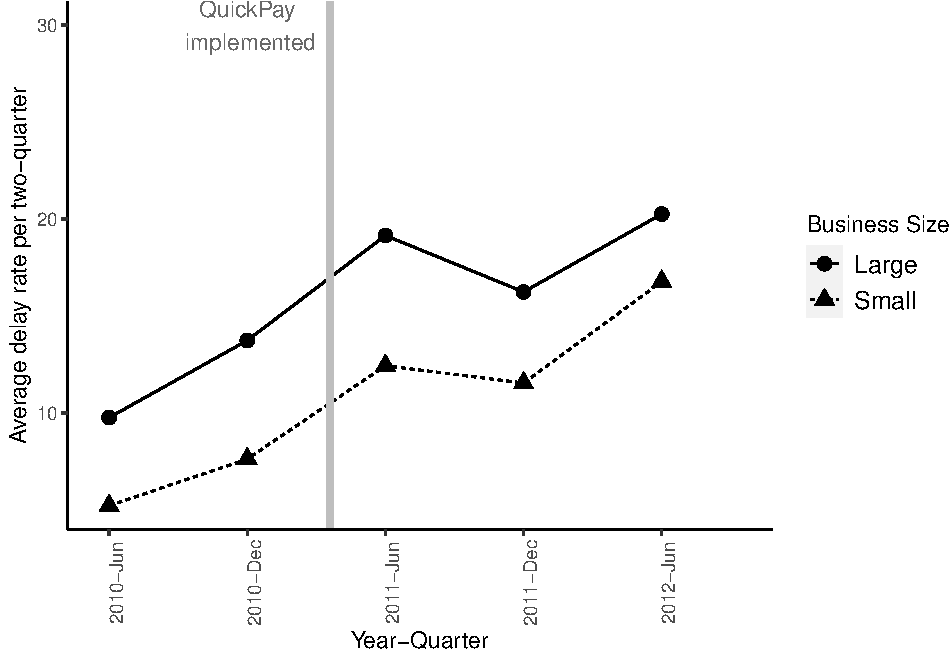
\includegraphics{qp_first_pc_delay_two_quarters_files/figure-latex/plot_pc_delay-1.pdf}

\hypertarget{normalized-delay-rate}{%
\subsection{Normalized delay rate}\label{normalized-delay-rate}}

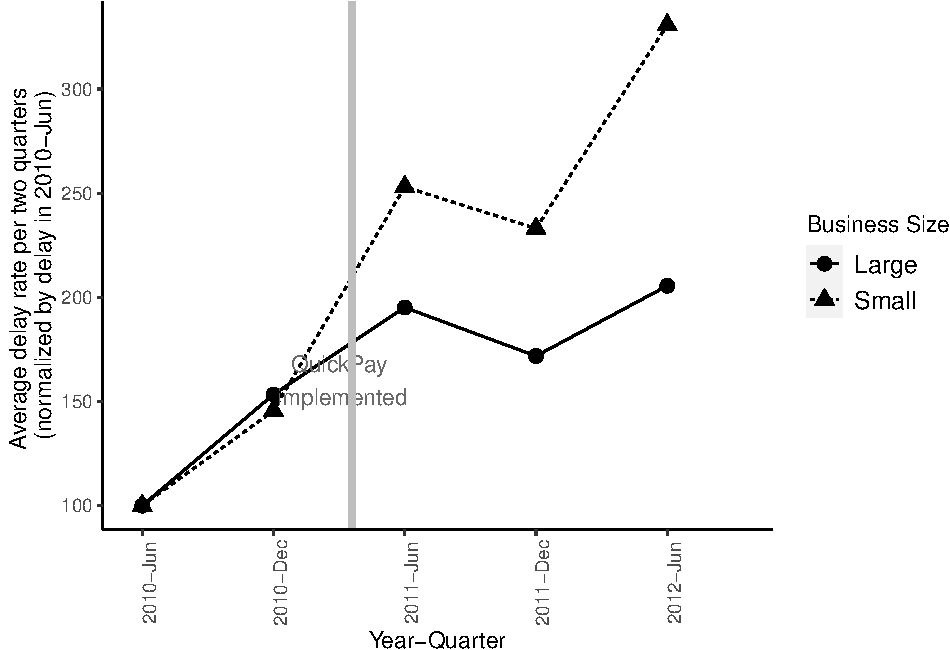
\includegraphics{qp_first_pc_delay_two_quarters_files/figure-latex/normalized_plot-1.pdf}

\hypertarget{full-sample-regressions}{%
\section{Full Sample Regressions}\label{full-sample-regressions}}

\hypertarget{winsorization}{%
\subsection{5\% Winsorization}\label{winsorization}}

\[ \begin{aligned} DelayRate_{it} &=& \alpha+\beta_0 Treat_i + \beta_1 Post_t + \beta_2 (Treat_i \times Post_t)\\
&+&  X_i + (Post_t \times X_i) + \mu_t + \theta_{firm} + \lambda_{task}+ \epsilon_{it}
\end{aligned}\]

\hypertarget{one-quarter}{%
\subsubsection{One Quarter}\label{one-quarter}}

\begin{table}[H] \centering 
  \caption{Effect of QuickPay on project delay rates} 
  \label{} 
\small 
\begin{tabular}{@{\extracolsep{-2pt}}lccccc} 
\\[-1.8ex]\hline 
\hline \\[-1.8ex] 
\\[-1.8ex] & \multicolumn{5}{c}{$DelayRate_{it}$} \\ 
\\[-1.8ex] & (1) & (2) & (3) & (4) & (5)\\ 
\hline \\[-1.8ex] 
 $Treat_i$ & $-$3.34$^{***}$ & $-$2.72$^{***}$ & $-$2.70$^{***}$ & $-$2.07$^{***}$ & $-$1.81$^{***}$ \\ 
  & (0.15) & (0.15) & (0.15) & (0.15) & (0.35) \\ 
  & & & & & \\ 
 $Post_t$ & 1.02$^{***}$ & $-$1.01$^{***}$ &  &  &  \\ 
  & (0.15) & (0.31) &  &  &  \\ 
  & & & & & \\ 
 $Treat_i \times Post_t$ & 1.34$^{***}$ & 1.62$^{***}$ & 1.62$^{***}$ & 1.33$^{***}$ & 1.51$^{***}$ \\ 
  & (0.19) & (0.20) & (0.20) & (0.19) & (0.21) \\ 
  & & & & & \\ 
 Constant & 8.35$^{***}$ & 16.93$^{***}$ &  &  &  \\ 
  & (0.12) & (0.24) &  &  &  \\ 
  & & & & & \\ 
\hline \\[-1.8ex] 
Duration, Budget, Bids & No & Yes & Yes & Yes & Yes \\ 
$Post_t \times$  (Duration, Budget, Bids) & No & Yes & Yes & Yes & Yes \\ 
Year-Quarter fixed effects & No & No & Yes & Yes & Yes \\ 
Task fixed effects & No & No & No & Yes & Yes \\ 
Contractor fixed effects & No & No & No & No & Yes \\ 
Observations & 287,530 & 263,488 & 263,488 & 263,488 & 263,488 \\ 
R$^{2}$ & 0.004 & 0.05 & 0.06 & 0.09 & 0.17 \\ 
Adjusted R$^{2}$ & 0.004 & 0.05 & 0.06 & 0.09 & 0.12 \\ 
\hline 
\hline \\[-1.8ex] 
\textit{Note:}  & \multicolumn{5}{r}{$^{*}$p$<$0.1; $^{**}$p$<$0.05; $^{***}$p$<$0.01} \\ 
 & \multicolumn{5}{r}{Each observation is a project-quarter.} \\ 
 & \multicolumn{5}{r}{SEs are robust and clustered at the project level.} \\ 
\end{tabular} 
\end{table}

\hypertarget{two-quarters}{%
\subsubsection{Two-Quarters}\label{two-quarters}}

\begin{table}[H] \centering 
  \caption{Effect of QuickPay on project delay rates} 
  \label{} 
\small 
\begin{tabular}{@{\extracolsep{-2pt}}lccccc} 
\\[-1.8ex]\hline 
\hline \\[-1.8ex] 
\\[-1.8ex] & \multicolumn{5}{c}{$DelayRate_{it}$} \\ 
\\[-1.8ex] & (1) & (2) & (3) & (4) & (5)\\ 
\hline \\[-1.8ex] 
 $Treat_i$ & $-$7.99$^{***}$ & $-$6.23$^{***}$ & $-$6.24$^{***}$ & $-$4.40$^{***}$ & $-$4.00$^{***}$ \\ 
  & (0.42) & (0.43) & (0.43) & (0.44) & (1.15) \\ 
  & & & & & \\ 
 $Post_t$ & 4.05$^{***}$ & $-$1.52 &  &  &  \\ 
  & (0.45) & (0.93) &  &  &  \\ 
  & & & & & \\ 
 $Treat_i \times Post_t$ & 2.57$^{***}$ & 3.36$^{***}$ & 3.37$^{***}$ & 2.64$^{***}$ & 3.25$^{***}$ \\ 
  & (0.56) & (0.59) & (0.60) & (0.59) & (0.66) \\ 
  & & & & & \\ 
 Constant & 19.65$^{***}$ & 36.57$^{***}$ &  &  &  \\ 
  & (0.34) & (0.67) &  &  &  \\ 
  & & & & & \\ 
\hline \\[-1.8ex] 
Duration, Budget, Bids & No & Yes & Yes & Yes & Yes \\ 
$Post_t \times$  (Duration, Budget, Bids) & No & Yes & Yes & Yes & Yes \\ 
Year-Quarter fixed effects & No & No & Yes & Yes & Yes \\ 
Task fixed effects & No & No & No & Yes & Yes \\ 
Contractor fixed effects & No & No & No & No & Yes \\ 
Observations & 122,172 & 111,681 & 111,681 & 111,681 & 111,681 \\ 
R$^{2}$ & 0.01 & 0.06 & 0.06 & 0.12 & 0.26 \\ 
Adjusted R$^{2}$ & 0.01 & 0.06 & 0.06 & 0.11 & 0.16 \\ 
\hline 
\hline \\[-1.8ex] 
\textit{Note:}  & \multicolumn{5}{r}{$^{*}$p$<$0.1; $^{**}$p$<$0.05; $^{***}$p$<$0.01} \\ 
 & \multicolumn{5}{r}{Each observation is a project-quarter.} \\ 
 & \multicolumn{5}{r}{SEs are robust and clustered at the project level.} \\ 
\end{tabular} 
\end{table}

\hypertarget{winsorization-1}{%
\subsection{2.5\% Winsorization}\label{winsorization-1}}

\[ \begin{aligned} DelayRate_{it} &=& \alpha+\beta_0 Treat_i + \beta_1 Post_t + \beta_2 (Treat_i \times Post_t)\\
&+&  X_i + (Post_t \times X_i) + \mu_t + \theta_{firm} + \lambda_{task}+ \epsilon_{it}
\end{aligned}\]

\hypertarget{one-quarter-1}{%
\subsubsection{One Quarter}\label{one-quarter-1}}

\begin{table}[H] \centering 
  \caption{Effect of QuickPay on project delay rates} 
  \label{} 
\small 
\begin{tabular}{@{\extracolsep{-2pt}}lccccc} 
\\[-1.8ex]\hline 
\hline \\[-1.8ex] 
\\[-1.8ex] & \multicolumn{5}{c}{$DelayRate_{it}$} \\ 
\\[-1.8ex] & (1) & (2) & (3) & (4) & (5)\\ 
\hline \\[-1.8ex] 
 $Treat_i$ & $-$5.22$^{***}$ & $-$4.32$^{***}$ & $-$4.30$^{***}$ & $-$3.21$^{***}$ & $-$2.64$^{***}$ \\ 
  & (0.23) & (0.24) & (0.24) & (0.24) & (0.56) \\ 
  & & & & & \\ 
 $Post_t$ & 2.22$^{***}$ & $-$0.48 &  &  &  \\ 
  & (0.24) & (0.49) &  &  &  \\ 
  & & & & & \\ 
 $Treat_i \times Post_t$ & 2.08$^{***}$ & 2.64$^{***}$ & 2.64$^{***}$ & 2.18$^{***}$ & 2.53$^{***}$ \\ 
  & (0.30) & (0.32) & (0.32) & (0.31) & (0.34) \\ 
  & & & & & \\ 
 Constant & 12.26$^{***}$ & 23.63$^{***}$ &  &  &  \\ 
  & (0.19) & (0.37) &  &  &  \\ 
  & & & & & \\ 
\hline \\[-1.8ex] 
Duration, Budget, Bids & No & Yes & Yes & Yes & Yes \\ 
$Post_t \times$  (Duration, Budget, Bids) & No & Yes & Yes & Yes & Yes \\ 
Year-Quarter fixed effects & No & No & Yes & Yes & Yes \\ 
Task fixed effects & No & No & No & Yes & Yes \\ 
Contractor fixed effects & No & No & No & No & Yes \\ 
Observations & 287,530 & 263,488 & 263,488 & 263,488 & 263,488 \\ 
R$^{2}$ & 0.004 & 0.04 & 0.04 & 0.07 & 0.14 \\ 
Adjusted R$^{2}$ & 0.004 & 0.04 & 0.04 & 0.07 & 0.09 \\ 
\hline 
\hline \\[-1.8ex] 
\textit{Note:}  & \multicolumn{5}{r}{$^{*}$p$<$0.1; $^{**}$p$<$0.05; $^{***}$p$<$0.01} \\ 
 & \multicolumn{5}{r}{Each observation is a project-quarter.} \\ 
 & \multicolumn{5}{r}{SEs are robust and clustered at the project level.} \\ 
\end{tabular} 
\end{table}

\hypertarget{two-quarters-1}{%
\subsubsection{Two-Quarters}\label{two-quarters-1}}

\begin{table}[H] \centering 
  \caption{Effect of QuickPay on project delay rates} 
  \label{} 
\small 
\begin{tabular}{@{\extracolsep{-2pt}}lccccc} 
\\[-1.8ex]\hline 
\hline \\[-1.8ex] 
\\[-1.8ex] & \multicolumn{5}{c}{$DelayRate_{it}$} \\ 
\\[-1.8ex] & (1) & (2) & (3) & (4) & (5)\\ 
\hline \\[-1.8ex] 
 $Treat_i$ & $-$10.70$^{***}$ & $-$8.44$^{***}$ & $-$8.46$^{***}$ & $-$5.53$^{***}$ & $-$5.31$^{***}$ \\ 
  & (0.59) & (0.62) & (0.62) & (0.63) & (1.73) \\ 
  & & & & & \\ 
 $Post_t$ & 6.48$^{***}$ & $-$1.54 &  &  &  \\ 
  & (0.64) & (1.32) &  &  &  \\ 
  & & & & & \\ 
 $Treat_i \times Post_t$ & 3.59$^{***}$ & 4.99$^{***}$ & 5.01$^{***}$ & 3.84$^{***}$ & 4.82$^{***}$ \\ 
  & (0.80) & (0.86) & (0.87) & (0.87) & (0.97) \\ 
  & & & & & \\ 
 Constant & 25.60$^{***}$ & 44.93$^{***}$ &  &  &  \\ 
  & (0.49) & (0.94) &  &  &  \\ 
  & & & & & \\ 
\hline \\[-1.8ex] 
Duration, Budget, Bids & No & Yes & Yes & Yes & Yes \\ 
$Post_t \times$  (Duration, Budget, Bids) & No & Yes & Yes & Yes & Yes \\ 
Year-Quarter fixed effects & No & No & Yes & Yes & Yes \\ 
Task fixed effects & No & No & No & Yes & Yes \\ 
Contractor fixed effects & No & No & No & No & Yes \\ 
Observations & 122,172 & 111,681 & 111,681 & 111,681 & 111,681 \\ 
R$^{2}$ & 0.01 & 0.04 & 0.05 & 0.10 & 0.23 \\ 
Adjusted R$^{2}$ & 0.01 & 0.04 & 0.05 & 0.09 & 0.13 \\ 
\hline 
\hline \\[-1.8ex] 
\textit{Note:}  & \multicolumn{5}{r}{$^{*}$p$<$0.1; $^{**}$p$<$0.05; $^{***}$p$<$0.01} \\ 
 & \multicolumn{5}{r}{Each observation is a project-quarter.} \\ 
 & \multicolumn{5}{r}{SEs are robust and clustered at the project level.} \\ 
\end{tabular} 
\end{table}

\hypertarget{truncation}{%
\subsection{2.5\% Truncation}\label{truncation}}

\[ \begin{aligned} DelayRate_{it} &=& \alpha+\beta_0 Treat_i + \beta_1 Post_t + \beta_2 (Treat_i \times Post_t)\\
&+&  X_i + (Post_t \times X_i) + \mu_t + \theta_{firm} + \lambda_{task}+ \epsilon_{it}
\end{aligned}\]

\hypertarget{one-quarter-2}{%
\subsubsection{One Quarter}\label{one-quarter-2}}

\begin{table}[H] \centering 
  \caption{Effect of QuickPay on project delay rates} 
  \label{} 
\small 
\begin{tabular}{@{\extracolsep{-2pt}}lccccc} 
\\[-1.8ex]\hline 
\hline \\[-1.8ex] 
\\[-1.8ex] & \multicolumn{5}{c}{$DelayRate_{it}$} \\ 
\\[-1.8ex] & (1) & (2) & (3) & (4) & (5)\\ 
\hline \\[-1.8ex] 
 $Treat_i$ & $-$13.85$^{***}$ & $-$13.95$^{***}$ & $-$14.13$^{***}$ & $-$12.74$^{***}$ & $-$12.31$^{***}$ \\ 
  & (1.17) & (1.17) & (1.16) & (1.23) & (4.26) \\ 
  & & & & & \\ 
 $Post_t$ & 1.56 & $-$2.00 &  &  &  \\ 
  & (1.04) & (1.44) &  &  &  \\ 
  & & & & & \\ 
 $Treat_i \times Post_t$ & 8.57$^{***}$ & 8.55$^{***}$ & 8.79$^{***}$ & 9.27$^{***}$ & 7.36$^{***}$ \\ 
  & (1.47) & (1.47) & (1.46) & (1.48) & (1.92) \\ 
  & & & & & \\ 
 Constant & 81.92$^{***}$ & 84.50$^{***}$ &  &  &  \\ 
  & (0.83) & (1.10) &  &  &  \\ 
  & & & & & \\ 
\hline \\[-1.8ex] 
Duration, Budget, Bids & No & Yes & Yes & Yes & Yes \\ 
$Post_t \times$  (Duration, Budget, Bids) & No & Yes & Yes & Yes & Yes \\ 
Year-Quarter fixed effects & No & No & Yes & Yes & Yes \\ 
Task fixed effects & No & No & No & Yes & Yes \\ 
Contractor fixed effects & No & No & No & No & Yes \\ 
Observations & 22,936 & 22,928 & 22,928 & 22,928 & 22,928 \\ 
R$^{2}$ & 0.01 & 0.01 & 0.02 & 0.11 & 0.37 \\ 
Adjusted R$^{2}$ & 0.01 & 0.01 & 0.02 & 0.08 & 0.17 \\ 
\hline 
\hline \\[-1.8ex] 
\textit{Note:}  & \multicolumn{5}{r}{$^{*}$p$<$0.1; $^{**}$p$<$0.05; $^{***}$p$<$0.01} \\ 
 & \multicolumn{5}{r}{Each observation is a project-quarter.} \\ 
 & \multicolumn{5}{r}{SEs are robust and clustered at the project level.} \\ 
\end{tabular} 
\end{table}

\hypertarget{two-quarters-2}{%
\subsubsection{Two-Quarters}\label{two-quarters-2}}

\begin{table}[H] \centering 
  \caption{Effect of QuickPay on project delay rates} 
  \label{} 
\small 
\begin{tabular}{@{\extracolsep{-2pt}}lccccc} 
\\[-1.8ex]\hline 
\hline \\[-1.8ex] 
\\[-1.8ex] & \multicolumn{5}{c}{$DelayRate_{it}$} \\ 
\\[-1.8ex] & (1) & (2) & (3) & (4) & (5)\\ 
\hline \\[-1.8ex] 
 $Treat_i$ & $-$19.48$^{***}$ & $-$19.26$^{***}$ & $-$19.25$^{***}$ & $-$17.02$^{***}$ & 1.95 \\ 
  & (2.12) & (2.10) & (2.09) & (2.21) & (9.19) \\ 
  & & & & & \\ 
 $Post_t$ & 9.12$^{***}$ & $-$4.09 &  &  &  \\ 
  & (1.93) & (2.80) &  &  &  \\ 
  & & & & & \\ 
 $Treat_i \times Post_t$ & 12.77$^{***}$ & 12.55$^{***}$ & 12.76$^{***}$ & 12.77$^{***}$ & 10.77$^{***}$ \\ 
  & (2.78) & (2.77) & (2.76) & (2.79) & (3.69) \\ 
  & & & & & \\ 
 Constant & 118.27$^{***}$ & 130.96$^{***}$ &  &  &  \\ 
  & (1.48) & (2.06) &  &  &  \\ 
  & & & & & \\ 
\hline \\[-1.8ex] 
Duration, Budget, Bids & No & Yes & Yes & Yes & Yes \\ 
$Post_t \times$  (Duration, Budget, Bids) & No & Yes & Yes & Yes & Yes \\ 
Year-Quarter fixed effects & No & No & Yes & Yes & Yes \\ 
Task fixed effects & No & No & No & Yes & Yes \\ 
Contractor fixed effects & No & No & No & No & Yes \\ 
Observations & 15,315 & 15,308 & 15,308 & 15,308 & 15,308 \\ 
R$^{2}$ & 0.01 & 0.02 & 0.02 & 0.14 & 0.46 \\ 
Adjusted R$^{2}$ & 0.01 & 0.02 & 0.02 & 0.09 & 0.22 \\ 
\hline 
\hline \\[-1.8ex] 
\textit{Note:}  & \multicolumn{5}{r}{$^{*}$p$<$0.1; $^{**}$p$<$0.05; $^{***}$p$<$0.01} \\ 
 & \multicolumn{5}{r}{Each observation is a project-quarter.} \\ 
 & \multicolumn{5}{r}{SEs are robust and clustered at the project level.} \\ 
\end{tabular} 
\end{table}

\hypertarget{sample-with-non-zero-delays}{%
\section{Sample with Non-Zero
Delays}\label{sample-with-non-zero-delays}}

\hypertarget{winsorization-on-full-sample}{%
\subsection{5\% winsorization on full
sample}\label{winsorization-on-full-sample}}

\[ \begin{aligned} DelayRate_{it} &=& \alpha+\beta_0 Treat_i + \beta_1 Post_t + \beta_2 (Treat_i \times Post_t)\\
&+&  X_i + (Post_t \times X_i) + \mu_t + \theta_{firm} + \lambda_{task}+ \epsilon_{it}
\end{aligned}\]

\hypertarget{one-quarter-3}{%
\subsubsection{One Quarter}\label{one-quarter-3}}

\begin{table}[H] \centering 
  \caption{Effect of QuickPay on project delay rates} 
  \label{} 
\small 
\begin{tabular}{@{\extracolsep{-2pt}}lccccc} 
\\[-1.8ex]\hline 
\hline \\[-1.8ex] 
\\[-1.8ex] & \multicolumn{5}{c}{$DelayRate_{it}$} \\ 
\\[-1.8ex] & (1) & (2) & (3) & (4) & (5)\\ 
\hline \\[-1.8ex] 
 $Treat_i$ & $-$9.22$^{***}$ & $-$9.34$^{***}$ & $-$9.38$^{***}$ & $-$7.62$^{***}$ & $-$5.47$^{***}$ \\ 
  & (0.69) & (0.69) & (0.68) & (0.70) & (2.11) \\ 
  & & & & & \\ 
 $Post_t$ & 2.29$^{***}$ & $-$0.51 &  &  &  \\ 
  & (0.54) & (0.78) &  &  &  \\ 
  & & & & & \\ 
 $Treat_i \times Post_t$ & 6.78$^{***}$ & 6.62$^{***}$ & 6.67$^{***}$ & 6.25$^{***}$ & 4.84$^{***}$ \\ 
  & (0.82) & (0.82) & (0.81) & (0.80) & (0.99) \\ 
  & & & & & \\ 
 Constant & 73.51$^{***}$ & 73.36$^{***}$ &  &  &  \\ 
  & (0.45) & (0.61) &  &  &  \\ 
  & & & & & \\ 
\hline \\[-1.8ex] 
Duration, Budget, Bids & No & Yes & Yes & Yes & Yes \\ 
$Post_t \times$  (Duration, Budget, Bids) & No & Yes & Yes & Yes & Yes \\ 
Year-Quarter fixed effects & No & No & Yes & Yes & Yes \\ 
Task fixed effects & No & No & No & Yes & Yes \\ 
Contractor fixed effects & No & No & No & No & Yes \\ 
Observations & 30,138 & 30,130 & 30,130 & 30,130 & 30,130 \\ 
R$^{2}$ & 0.01 & 0.02 & 0.03 & 0.14 & 0.39 \\ 
Adjusted R$^{2}$ & 0.01 & 0.02 & 0.03 & 0.11 & 0.21 \\ 
\hline 
\hline \\[-1.8ex] 
\textit{Note:}  & \multicolumn{5}{r}{$^{*}$p$<$0.1; $^{**}$p$<$0.05; $^{***}$p$<$0.01} \\ 
 & \multicolumn{5}{r}{Each observation is a project-quarter.} \\ 
 & \multicolumn{5}{r}{SEs are robust and clustered at the project level.} \\ 
\end{tabular} 
\end{table}

\hypertarget{two-quarters-3}{%
\subsubsection{Two Quarters}\label{two-quarters-3}}

\begin{table}[H] \centering 
  \caption{Effect of QuickPay on project delay rates} 
  \label{} 
\small 
\begin{tabular}{@{\extracolsep{-2pt}}lccccc} 
\\[-1.8ex]\hline 
\hline \\[-1.8ex] 
\\[-1.8ex] & \multicolumn{5}{c}{$DelayRate_{it}$} \\ 
\\[-1.8ex] & (1) & (2) & (3) & (4) & (5)\\ 
\hline \\[-1.8ex] 
 $Treat_i$ & $-$16.47$^{***}$ & $-$16.73$^{***}$ & $-$16.59$^{***}$ & $-$12.45$^{***}$ & $-$4.57 \\ 
  & (1.60) & (1.60) & (1.59) & (1.64) & (5.65) \\ 
  & & & & & \\ 
 $Post_t$ & 9.03$^{***}$ & $-$0.10 &  &  &  \\ 
  & (1.33) & (2.00) &  &  &  \\ 
  & & & & & \\ 
 $Treat_i \times Post_t$ & 11.55$^{***}$ & 11.12$^{***}$ & 11.09$^{***}$ & 10.11$^{***}$ & 7.81$^{***}$ \\ 
  & (1.97) & (1.97) & (1.96) & (1.95) & (2.51) \\ 
  & & & & & \\ 
 Constant & 119.88$^{***}$ & 122.61$^{***}$ &  &  &  \\ 
  & (1.08) & (1.53) &  &  &  \\ 
  & & & & & \\ 
\hline \\[-1.8ex] 
Duration, Budget, Bids & No & Yes & Yes & Yes & Yes \\ 
$Post_t \times$  (Duration, Budget, Bids) & No & Yes & Yes & Yes & Yes \\ 
Year-Quarter fixed effects & No & No & Yes & Yes & Yes \\ 
Task fixed effects & No & No & No & Yes & Yes \\ 
Contractor fixed effects & No & No & No & No & Yes \\ 
Observations & 18,616 & 18,609 & 18,609 & 18,609 & 18,609 \\ 
R$^{2}$ & 0.02 & 0.03 & 0.03 & 0.18 & 0.48 \\ 
Adjusted R$^{2}$ & 0.02 & 0.02 & 0.03 & 0.14 & 0.26 \\ 
\hline 
\hline \\[-1.8ex] 
\textit{Note:}  & \multicolumn{5}{r}{$^{*}$p$<$0.1; $^{**}$p$<$0.05; $^{***}$p$<$0.01} \\ 
 & \multicolumn{5}{r}{Each observation is a project-quarter.} \\ 
 & \multicolumn{5}{r}{SEs are robust and clustered at the project level.} \\ 
\end{tabular} 
\end{table}

\hypertarget{winsorization-on-non-zero-sample}{%
\subsection{2.5\% winsorization on non-zero
sample}\label{winsorization-on-non-zero-sample}}

\[ \begin{aligned} DelayRate_{it} &=& \alpha+\beta_0 Treat_i + \beta_1 Post_t + \beta_2 (Treat_i \times Post_t)\\
&+&  X_i + (Post_t \times X_i) + \mu_t + \theta_{firm} + \lambda_{task}+ \epsilon_{it}
\end{aligned}\]

\hypertarget{one-quarter-4}{%
\subsubsection{One Quarter}\label{one-quarter-4}}

\begin{table}[H] \centering 
  \caption{Effect of QuickPay on project delay rates} 
  \label{} 
\small 
\begin{tabular}{@{\extracolsep{-2pt}}lccccc} 
\\[-1.8ex]\hline 
\hline \\[-1.8ex] 
\\[-1.8ex] & \multicolumn{5}{c}{$DelayRate_{it}$} \\ 
\\[-1.8ex] & (1) & (2) & (3) & (4) & (5)\\ 
\hline \\[-1.8ex] 
 $Treat_i$ & $-$24.72$^{***}$ & $-$24.71$^{***}$ & $-$24.59$^{***}$ & $-$15.28$^{***}$ & $-$16.40$^{*}$ \\ 
  & (2.43) & (2.44) & (2.42) & (2.49) & (8.45) \\ 
  & & & & & \\ 
 $Post_t$ & 15.46$^{***}$ & 3.48 &  &  &  \\ 
  & (2.15) & (2.95) &  &  &  \\ 
  & & & & & \\ 
 $Treat_i \times Post_t$ & 25.24$^{***}$ & 24.34$^{***}$ & 24.07$^{***}$ & 22.04$^{***}$ & 18.45$^{***}$ \\ 
  & (3.07) & (3.07) & (3.05) & (3.03) & (3.87) \\ 
  & & & & & \\ 
 Constant & 118.01$^{***}$ & 124.90$^{***}$ &  &  &  \\ 
  & (1.72) & (2.22) &  &  &  \\ 
  & & & & & \\ 
\hline \\[-1.8ex] 
Duration, Budget, Bids & No & Yes & Yes & Yes & Yes \\ 
$Post_t \times$  (Duration, Budget, Bids) & No & Yes & Yes & Yes & Yes \\ 
Year-Quarter fixed effects & No & No & Yes & Yes & Yes \\ 
Task fixed effects & No & No & No & Yes & Yes \\ 
Contractor fixed effects & No & No & No & No & Yes \\ 
Observations & 32,707 & 32,699 & 32,699 & 32,699 & 32,699 \\ 
R$^{2}$ & 0.01 & 0.02 & 0.02 & 0.14 & 0.40 \\ 
Adjusted R$^{2}$ & 0.01 & 0.02 & 0.02 & 0.12 & 0.23 \\ 
\hline 
\hline \\[-1.8ex] 
\textit{Note:}  & \multicolumn{5}{r}{$^{*}$p$<$0.1; $^{**}$p$<$0.05; $^{***}$p$<$0.01} \\ 
 & \multicolumn{5}{r}{Each observation is a project-quarter.} \\ 
 & \multicolumn{5}{r}{SEs are robust and clustered at the project level.} \\ 
\end{tabular} 
\end{table}

\hypertarget{two-quarters-4}{%
\subsubsection{Two Quarters}\label{two-quarters-4}}

\begin{table}[H] \centering 
  \caption{Effect of QuickPay on project delay rates} 
  \label{} 
\small 
\begin{tabular}{@{\extracolsep{-2pt}}lccccc} 
\\[-1.8ex]\hline 
\hline \\[-1.8ex] 
\\[-1.8ex] & \multicolumn{5}{c}{$DelayRate_{it}$} \\ 
\\[-1.8ex] & (1) & (2) & (3) & (4) & (5)\\ 
\hline \\[-1.8ex] 
 $Treat_i$ & $-$26.92$^{***}$ & $-$26.68$^{***}$ & $-$26.37$^{***}$ & $-$16.57$^{***}$ & $-$9.57 \\ 
  & (3.28) & (3.27) & (3.25) & (3.35) & (12.35) \\ 
  & & & & & \\ 
 $Post_t$ & 19.70$^{***}$ & 3.33 &  &  &  \\ 
  & (2.95) & (4.34) &  &  &  \\ 
  & & & & & \\ 
 $Treat_i \times Post_t$ & 24.39$^{***}$ & 23.17$^{***}$ & 23.12$^{***}$ & 21.01$^{***}$ & 18.96$^{***}$ \\ 
  & (4.26) & (4.24) & (4.22) & (4.20) & (5.58) \\ 
  & & & & & \\ 
 Constant & 145.54$^{***}$ & 164.54$^{***}$ &  &  &  \\ 
  & (2.29) & (3.14) &  &  &  \\ 
  & & & & & \\ 
\hline \\[-1.8ex] 
Duration, Budget, Bids & No & Yes & Yes & Yes & Yes \\ 
$Post_t \times$  (Duration, Budget, Bids) & No & Yes & Yes & Yes & Yes \\ 
Year-Quarter fixed effects & No & No & Yes & Yes & Yes \\ 
Task fixed effects & No & No & No & Yes & Yes \\ 
Contractor fixed effects & No & No & No & No & Yes \\ 
Observations & 20,072 & 20,065 & 20,065 & 20,065 & 20,065 \\ 
R$^{2}$ & 0.01 & 0.02 & 0.02 & 0.17 & 0.47 \\ 
Adjusted R$^{2}$ & 0.01 & 0.02 & 0.02 & 0.13 & 0.25 \\ 
\hline 
\hline \\[-1.8ex] 
\textit{Note:}  & \multicolumn{5}{r}{$^{*}$p$<$0.1; $^{**}$p$<$0.05; $^{***}$p$<$0.01} \\ 
 & \multicolumn{5}{r}{Each observation is a project-quarter.} \\ 
 & \multicolumn{5}{r}{SEs are robust and clustered at the project level.} \\ 
\end{tabular} 
\end{table}

\hypertarget{truncation-on-non-zero-sample}{%
\subsection{2.5\% truncation on non-zero
sample}\label{truncation-on-non-zero-sample}}

\[ \begin{aligned} DelayRate_{it} &=& \alpha+\beta_0 Treat_i + \beta_1 Post_t + \beta_2 (Treat_i \times Post_t)\\
&+&  X_i + (Post_t \times X_i) + \mu_t + \theta_{firm} + \lambda_{task}+ \epsilon_{it}
\end{aligned}\]

\hypertarget{one-quarter-5}{%
\subsubsection{One Quarter}\label{one-quarter-5}}

\begin{table}[H] \centering 
  \caption{Effect of QuickPay on project delay rates} 
  \label{} 
\small 
\begin{tabular}{@{\extracolsep{-2pt}}lccccc} 
\\[-1.8ex]\hline 
\hline \\[-1.8ex] 
\\[-1.8ex] & \multicolumn{5}{c}{$DelayRate_{it}$} \\ 
\\[-1.8ex] & (1) & (2) & (3) & (4) & (5)\\ 
\hline \\[-1.8ex] 
 $Treat_i$ & $-$21.36$^{***}$ & $-$21.92$^{***}$ & $-$21.86$^{***}$ & $-$12.74$^{***}$ & $-$11.93 \\ 
  & (2.22) & (2.23) & (2.21) & (2.24) & (7.45) \\ 
  & & & & & \\ 
 $Post_t$ & 14.90$^{***}$ & $-$0.49 &  &  &  \\ 
  & (1.88) & (2.59) &  &  &  \\ 
  & & & & & \\ 
 $Treat_i \times Post_t$ & 20.83$^{***}$ & 19.85$^{***}$ & 19.74$^{***}$ & 17.79$^{***}$ & 13.93$^{***}$ \\ 
  & (2.73) & (2.72) & (2.71) & (2.67) & (3.27) \\ 
  & & & & & \\ 
 Constant & 116.26$^{***}$ & 112.31$^{***}$ &  &  &  \\ 
  & (1.55) & (2.02) &  &  &  \\ 
  & & & & & \\ 
\hline \\[-1.8ex] 
Duration, Budget, Bids & No & Yes & Yes & Yes & Yes \\ 
$Post_t \times$  (Duration, Budget, Bids) & No & Yes & Yes & Yes & Yes \\ 
Year-Quarter fixed effects & No & No & Yes & Yes & Yes \\ 
Task fixed effects & No & No & No & Yes & Yes \\ 
Contractor fixed effects & No & No & No & No & Yes \\ 
Observations & 31,069 & 31,061 & 31,061 & 31,061 & 31,061 \\ 
R$^{2}$ & 0.01 & 0.03 & 0.04 & 0.18 & 0.46 \\ 
Adjusted R$^{2}$ & 0.01 & 0.03 & 0.04 & 0.15 & 0.30 \\ 
\hline 
\hline \\[-1.8ex] 
\textit{Note:}  & \multicolumn{5}{r}{$^{*}$p$<$0.1; $^{**}$p$<$0.05; $^{***}$p$<$0.01} \\ 
 & \multicolumn{5}{r}{Each observation is a project-quarter.} \\ 
 & \multicolumn{5}{r}{SEs are robust and clustered at the project level.} \\ 
\end{tabular} 
\end{table}

\hypertarget{two-quarters-5}{%
\subsubsection{Two Quarters}\label{two-quarters-5}}

\begin{itemize}
\tightlist
\item
  2.5\% truncation done after calculating 2Q delays
\end{itemize}

\begin{table}[H] \centering 
  \caption{Effect of QuickPay on project delay rates} 
  \label{} 
\small 
\begin{tabular}{@{\extracolsep{-2pt}}lccccc} 
\\[-1.8ex]\hline 
\hline \\[-1.8ex] 
\\[-1.8ex] & \multicolumn{5}{c}{$DelayRate_{it}$} \\ 
\\[-1.8ex] & (1) & (2) & (3) & (4) & (5)\\ 
\hline \\[-1.8ex] 
 $Treat_i$ & $-$23.80$^{***}$ & $-$24.32$^{***}$ & $-$24.05$^{***}$ & $-$13.92$^{***}$ & $-$9.25 \\ 
  & (2.93) & (2.91) & (2.90) & (2.93) & (11.08) \\ 
  & & & & & \\ 
 $Post_t$ & 18.68$^{***}$ & $-$2.33 &  &  &  \\ 
  & (2.52) & (3.68) &  &  &  \\ 
  & & & & & \\ 
 $Treat_i \times Post_t$ & 21.79$^{***}$ & 20.65$^{***}$ & 20.61$^{***}$ & 18.79$^{***}$ & 15.81$^{***}$ \\ 
  & (3.67) & (3.66) & (3.64) & (3.61) & (4.64) \\ 
  & & & & & \\ 
 Constant & 142.46$^{***}$ & 148.21$^{***}$ &  &  &  \\ 
  & (2.03) & (2.79) &  &  &  \\ 
  & & & & & \\ 
\hline \\[-1.8ex] 
Duration, Budget, Bids & No & Yes & Yes & Yes & Yes \\ 
$Post_t \times$  (Duration, Budget, Bids) & No & Yes & Yes & Yes & Yes \\ 
Year-Quarter fixed effects & No & No & Yes & Yes & Yes \\ 
Task fixed effects & No & No & No & Yes & Yes \\ 
Contractor fixed effects & No & No & No & No & Yes \\ 
Observations & 19,065 & 19,058 & 19,058 & 19,058 & 19,058 \\ 
R$^{2}$ & 0.01 & 0.03 & 0.03 & 0.20 & 0.51 \\ 
Adjusted R$^{2}$ & 0.01 & 0.03 & 0.03 & 0.17 & 0.31 \\ 
\hline 
\hline \\[-1.8ex] 
\textit{Note:}  & \multicolumn{5}{r}{$^{*}$p$<$0.1; $^{**}$p$<$0.05; $^{***}$p$<$0.01} \\ 
 & \multicolumn{5}{r}{Each observation is a project-quarter.} \\ 
 & \multicolumn{5}{r}{SEs are robust and clustered at the project level.} \\ 
\end{tabular} 
\end{table}

\end{document}
